\documentclass[conference]{IEEEtran}

% Packages for pt-BR spelling
\usepackage[utf8]{inputenc}
\usepackage[T1]{fontenc}
\usepackage[english, portuguese]{babel}
\usepackage{hyphenat}
\hyphenation{mate-mática recu-perar}
\usepackage{cite}
\usepackage {times}	
\usepackage {latexsym}		
\usepackage {alltt}	
\usepackage {fancyhdr}	
\usepackage {indentfirst}		  
\usepackage {vmargin}
\usepackage[table,xcdraw]{xcolor}
\usepackage{algorithmic}
\usepackage{algorithm}
\usepackage{clrscode}
\usepackage{float}
\usepackage[normal]{subfigure} 
\usepackage[normalem]{ulem}
\usepackage{wrapfig}
\usepackage{amsmath}
\usepackage{graphicx}
\usepackage{pgfplots}
\graphicspath{ {imagens/} }
\usepackage{float}
\usepackage{environ}
\usepackage{verbatim}
%\usepackage[num]{abntex2cite}
\usepackage{verbatim}
\usepackage{enumerate}
\usepackage{booktabs}
\usepackage{listings}
\usepackage{textcomp}
\definecolor{listinggray}{gray}{0.9}
\definecolor{lbcolor}{rgb}{1,1,1}
\lstset{
	backgroundcolor=\color{lbcolor},
	tabsize=3,
	rulecolor=,
	language=SQL,
        basicstyle=\small,
        upquote=true,
        aboveskip={1\baselineskip},
        columns=fixed,
        showstringspaces=false,
        extendedchars=true,
        breaklines=true,
        prebreak = \raisebox{0ex}[0ex][0ex]{\ensuremath{\hookleftarrow}},
        showtabs=false,
        showspaces=false,
        showstringspaces=false,
        identifierstyle=\ttfamily,
				numbers=left,
        numberstyle=\tiny,
        keywordstyle=\color[rgb]{0,0,1},
        commentstyle=\color[rgb]{0.133,0.545,0.133},
        stringstyle=\color[rgb]{0.627,0.126,0.941},
}

\NewEnviron{myequation}{%
\begin{equation}
\scalebox{1.5}{$\BODY$}
\end{equation}
}

\usepackage{color}
\usepackage{booktabs}


\begin{document}


%
% paper title
% Titles are generally capitalized except for words such as a, an, and, as,
% at, but, by, for, in, nor, of, on, or, the, to and up, which are usually
% not capitalized unless they are the first or last word of the title.
% Linebreaks \\ can be used within to get better formatting as desired.
% Do not put math or special symbols in the title.
\title{Avaliando o Impacto da Modelagem de Dados em Aplicações OLAP Utilizando SGBD Relacional e Colunar}


% author names and affiliations
% use a multiple column layout for up to three different
% affiliations
% \author{\IEEEauthorblockN{Clodis Boscarioli}
% \IEEEauthorblockA{Ciência da Computação\\Universidade Estadual do Oeste do Paraná\\
% Cascavel - PR, Brasil 85819--110\\
% Email: }
% \and
% \IEEEauthorblockN{Letícia Torres}
% \IEEEauthorblockA{Ciência da Computação\\Universidade Estadual do Oeste do Paraná\\
% Cascavel - PR, Brasil 85819--110\\
% Email: }
% }

% for over three affiliations, or if they all won't fit within the width
% of the page, use this alternative format:
% 
%\author{\IEEEauthorblockN{Michael Shell\IEEEauthorrefmark{1},
%Homer Simpson\IEEEauthorrefmark{2},
%James Kirk\IEEEauthorrefmark{3}, 
%Montgomery Scott\IEEEauthorrefmark{3} and
%Eldon Tyrell\IEEEauthorrefmark{4}}
%\IEEEauthorblockA{\IEEEauthorrefmark{1}School of Electrical and Computer Engineering\\
%Georgia Institute of Technology,
%Atlanta, Georgia 30332--0250\\ Email: see http://www.michaelshell.org/contact.html}
%\IEEEauthorblockA{\IEEEauthorrefmark{2}Twentieth Century Fox, Springfield, USA\\
%Email: homer@thesimpsons.com}
%\IEEEauthorblockA{\IEEEauthorrefmark{3}Starfleet Academy, San Francisco, California 96678-2391\\
%Telephone: (800) 555--1212, Fax: (888) 555--1212}
%\IEEEauthorblockA{\IEEEauthorrefmark{4}Tyrell Inc., 123 Replicant Street, Los Angeles, California 90210--4321}}


% use for special paper notices
%\IEEEspecialpapernotice{(Invited Paper)}




% make the title area
\maketitle
\selectlanguage{english}
\begin{abstract}
Data Warehouses has consolidate as the decision support technology used by Organizations that uses OLAP applications to access the stored data. As these data volume increases more efficient approaches to process them are needed. To do so, both relational databases management systems and NoSQL can be used, each one with their advantages over the Data Warehouse modeling. More normalized models are traditional among relational databases, whereas denormalized ones bring a better performance in NoSQL DBMS. A comparative study between PostgreSQL and MonetDB DBMS using TPC-H as a benchmark is presented here, to investigate which one is indicated to manage a Data Warehouse in information access. The results confirmed that, isolated, in denormalized environments MonetDB excels, while PostgreSQL is  better for normalized modeling. In general, MonetDB stands out compared to PostgreSQL, wich gains of almost 500\% on normalized model, and over 1000\% on the denormalized one.
\end{abstract}

\selectlanguage{portuguese}
\begin{abstract}
Data Warehouses se consolidaram nas Organizações como tecnologia de apoio à tomada de decisão utilizando aplicações OLAP sobre os dados armazenados. Conforme o volume destes dados aumenta, tornam-se necessárias abordagens mais eficientes para seu processamento. Para tal tanto sistemas gerenciadores de banco de dados relacionais quanto NoSQL podem ser utilizados, e cada qual tem suas vantagens conforme a modelagem do Data Warehouse. Modelagens mais normalizadas são tradicionais entre os relacionais, enquanto que modelagens denormalizadas trazem desempenho superior em SGBD NoSQL. Um estudo comparativo entre os SGBD PostgreSQL e MonetDB utilizando o TPC-H como benchmark é aqui apresentado, investigando qual é o mais indicado para gerenciar um Data Warehouse na recuperação de informações. Os resultados experimentais confirmam que, isoladamente, em ambientes denormalizados o MonetDB se destaca, enquanto que o PostgreSQL é melhor em ambientes normalizados. Como um todo o MonetDB mostrou-se superior ao PostgreSQL obtendo ganhos de quase 500\% para o modelo normalizado e superior a 1000\% para o denormalizado.
\end{abstract}

\IEEEpeerreviewmaketitle

\tikzstyle{block} = [rectangle, draw, 
    text centered, rounded corners, minimum height=1cm]
\tikzstyle{line} = [draw, -latex']


\section{Introdução}

Organizações cada vez mais se apoiam no armazenamento de dados a fim de recuperar informações para tomadas de decisões de maneira ágil e eficaz. Estes dados são mantidos ao longo do tempo e por vezes são armazenados em sistemas que diminuem a eficiência no acesso e processamento de dados por serem heterogêneos, autônomos e geograficamente distribuídos \cite{wrembel2007data}.

Como forma de tratar um grande volume de dados, persisti-los e tomar decisões de maneira inteligente e eficiente a tecnologia de Data Warehouse é aplicada. Esta tecnologia consiste em um repositório de dados homogêneo, local e centralizado capaz de fornecer informações de diversas fontes de dados \cite{wrembel2007data}; e seu conceito está atrelado a criação de um ambiente com acesso a dados para tomar decisões de forma rápida e efetiva.

Para uma boa decisão de negócio além de um repositório é necessário uma aplicação que o acesse e traga informações. Aplicações OLAP (\textit{Online Analytical Processing}) estão fortemente associadas a Data Warehouses por tratarem de uma análise multidimensional de dados e consultas analíticas. À combinação de um Data Warehouse e aplicações OLAP dá-se o nome de ambiente OLAP.

Existe uma série de princípios que devem ser seguidos ao projetar e implantar um ambiente OLAP, destacando-se a rapidez com que os dados devem ser recuperados \cite{codd1998providing, kimball2002dw, wrembel2007data}. Assim, um dos aspectos técnicos a ser considerado é o uso de Sistemas Gerenciadores de Bancos de Dados (SGBD) como gerenciadores de um Data Warehouse, e duas classes de SGBD podem ser utilizadas para implementar este ambiente: SGBD relacionais e NoSQL. Dada a importância na escolha de um SGBD e as diferentes soluções apresentadas por cada um é viável o uso de um benchmark para a análise e conclusão de qual SGBD escolher. Tendo em vista o escopo da decisão de negócio, busca-se um benchmark que englobe e trabalhe com foco nisto e que traga uma configuração que se aplique tanto em SGBD relacionais quanto NoSQL. Com esse objetivo, a organização TPC \cite{tpc2017page} desenvolveu um benchmark para avaliar o desempenho de SGBD atuando em ambiente OLAP, o TPC-H \cite{tpch2017page}. 

Além dos SGBD, deve-se considerar ainda o ambiente para análise de dados. Segundo Bax e Souza \cite{bax2003modelagem} algumas empresas utilizam um ambiente normalizado devido a facilidade de manutenção, pelo fácil entendimento da relação entre as entidades e atributos e uma visão mais clara do sistema; por outro lado, modelos denormalizados são bastante utilizados devido ao ganho de desempenho nas consultas, pela diminuição do número de entidades e por consequência das operações de junção entre as tabelas.

Dadas as variáveis SGBD relacional e NoSQL, bem como ambientes com modelagem denormalizada e normalizada, o objetivo aqui é realizar um estudo comparativo entre SGBD como gerenciadores de um Data Warehouse utilizando-se de um benchmark. Os SGBD escolhidos foram o PostgreSQL como relacional, devido a sua ampla utilização no mercado, boa documentação e uso da linguagem SQL sem muitas modificações; e o MonetDB como NoSQL, por ainda utilizar-se da linguagem SQL, possuir interface simples através de linhas de comando, e ser o pioneiro entre os bancos NoSQL colunares.

\section{Persistência de Dados e Recuperação de Informações}

Como mencionado, empresas estão cada vez mais se apoiando na tomada de decisões a partir de dados persistidos em seus Data Warehouses. Inmon \cite{inmon2005building} define um Data Warehouse como base de todos os sistemas de suporte a decisão, atualmente definido como ambiente OLAP, e ainda como sendo uma coleção de dados não-volátil, orientado ao assunto principal da organização, integrado e variante no tempo. Estruturalmente, o repositório é definido como uma base de dados homogênea, local e centralizada \cite{wrembel2007data}.

Para analisar os dados armazenados no Data Warehouse além de implementá-lo é necessário que alguma aplicação leia seu conteúdo e apresente-o de forma gráfica e intuitiva ao analisador. Aplicações OLTP (\textit{Online Transaction Processing}) são amplamente utilizadas por bancos operacionais através de transações que seguem o conceito de ACID -- atomicidade, consistência, isolamento e durabilidade; entretanto, Data Warehouses trabalham com uma grande massa de dados, suporte a decisão e são intensivos para consultas analíticas, que acessam milhões de registros \cite{chaudhuri1997overview}, combinando diversos dados a fim de retornar uma informação útil para o mercado. Sendo assim, dados históricos armazenados ao longo do tempo na empresa, taxa de vazão de consultas e, sobretudo, o tempo de resposta são mais importantes que pequenas transações. 

Fugindo um pouco da ideia de ACID, aplicações OLAP se aplicam melhor no contexto apresentado por não focarem em pequenas transações. Elas têm por objetivo identificar tendências, padrões de comportamento e anomalias, bem como relações entre dados aparentemente não relacionados \cite{codd1998providing} sob um grande volume de dados. Geralmente as consultas em uma aplicação analítica são longas, levam tempo para executar e estão interessadas em atributos específicos. Ainda, o processo de inserção de dados em um ambiente OLAP é um pouco mais complexo que sistemas OLTP por seguir um processo fim-a-fim conhecido como ETL (extração, transformação e carga) \cite{vertabelo2017olap}

O processo ETL faz parte da arquitetura de um Data Warehouse, e consiste em \textit{extrair} dados de fontes heterogêneas para inseri-los em uma área de armazenamento temporária, denominada \textit{staging area}, onde então será feita uma \textit{transformação} de dados -- limpeza, homogeneização, remoção de redundância e atribuição de chaves aos dados, de acordo com a modelagem do Data Warehouse; e por fim o \textit{carregamento} dos registros na área de estruturação, que consiste no Data Warehouse em si. Esta área de estruturação trata de como os dados serão organizados, armazenados e disponibilizados para as aplicações analíticas, e é nela que a modelagem conceitual é definida.

Normalmente bancos operacionais utilizam a tradicional modelagem relacional normalizada até a Terceira Forma Normal. Aplicações OLAP têm por base a modelagem dimensional, ou multidimensional, que faz uma analogia com um cubo para representar seus dados, uma vez que uma informação pode ser vista através de \textit{n} dimensões.

% \begin{figure*}[htpb]
% 	\centering
% 		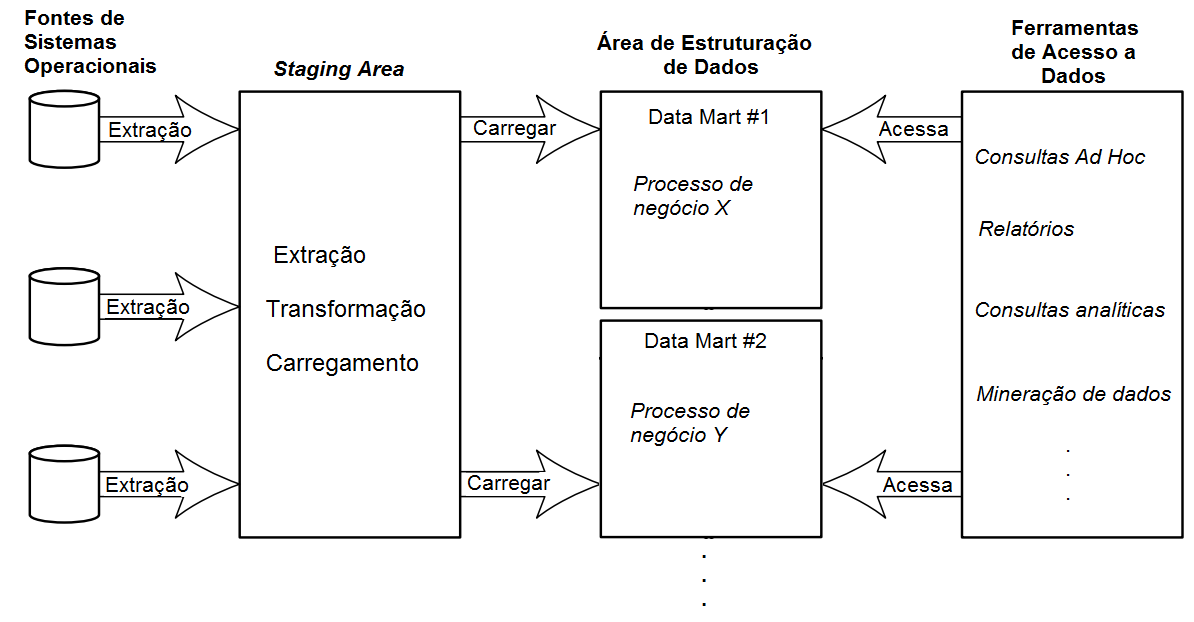
\includegraphics[width=\textwidth]{imagens/dw_arc}
% 	\caption{Arquitetura de um Data Warehouse}
% 	\label{fig:dw_arq}
% \end{figure*}


\subsection{Modelagem Dimensional}

Enquanto que uma aplicação OLTP visa um alto nível de normalização, aplicações OLAP priorizam desempenho e portanto um nível maior de denormalização. Ainda não há, porém, consenso acerca da modelagem conceitual no campo do Data Warehouse \cite{sen2005comparison}. Apesar disso, a modelagem Entidade-Relacional é voltada para consultas que realizam associações entre dados ao invés de consultas analíticas \cite{kimball2002dw} que visam construir e trazer maior clareza sobre cenários de decisão.

Em sua concepção, a modelagem dimensional é composta por tabelas fato e tabelas dimensão.

\subsubsection{Tabelas Fato}

De acordo com Kimball \cite{kimball2002dw}, uma tabela fato, ou apenas fato, traz a lista de atributos que representam as regras, ou métricas, de negócio. Fatos geralmente são descritos como atributos numéricos, relacionados com quantidades; e aditivos, pois uma aplicação OLAP nunca irá retornar somente uma tupla fato, mas sim várias tuplas onde a operação mais recorrente é a soma de todas elas.

Atributos textuais não são definidos como um fato. Na maioria das vezes descrevem algo e devem estar inseridos em tabelas dimensão pois há maior chance de estarem relacionados com os atributos dimensão e consomem menos espaço em disco. Outro ponto a se ater é a importância de se evitar incluir dados com zeros que não representam dados úteis, ou representando nada, pois a inclusão de dados sem significado sobrecarregariam o Data Warehouse sem motivo.

\subsubsection{Tabelas Dimensão}
Como dito, tabelas fato não trazem consigo atributos textuais de negócio, apenas métricas. As entidades responsáveis por isto são as entidades dimensão, que contém descrições que tornam os fatos mais claros. Não é estranho encontrar tabelas com mais de 100 atributos e poucas tuplas, pois a intenção das dimensões é descrever as regras de negócio.

É nas tabelas dimensão que são realizados os filtros de consulta. Por filtros, entende-se agrupamentos, padrões e ordenações por exemplo. De forma a exemplificar, se fosse desejado buscar as vendas por nome de fornecedor em um determinado intervalo de data, os atributos "nome de fornecedor" e "data" deveriam estar armazenados em tabelas dimensão. Segundo Kimball \cite{kimball2002dw}, quanto mais bem descritos os atributos dimensão, melhor o Data Warehouse é, tornando a qualidade do Warehouse dependente das entidades de dimensão.


Os modelos dimensionais compostos por tabelas fato e dimensão aplicados no escopo do warehouse são comumente conhecidos como modelos estrela (modelos \textit{star}, ou \textit{star join}) \cite{wrembel2007data, kimball2002dw, inmon2005building,sen2005comparison}, pois é organizado de forma a ter um único fato com várias dimensões. Este modelo torna a modelagem simples, trazendo benefícios ao desempenho na recuperação de dados devido a redução no número de junções; ademais, é flexível à alterações e expansões.

Com a afirmação de que modelos normalizados são mais fáceis para se dar manutenção não sendo necessário, por exemplo, alterar exaustivamente vários registros de um atributo em uma relação pois ele não será repetido, alguns modelos \textit{star} podem ser trabalhados para oferecer suporte à hierarquia de atributos das tabelas dimensões, criando novas tabelas denominadas subdimensão. Estes modelos \textit{star-normalizados} são conhecidos como \textit{snowflake} e caracterizam bem modelos relacionais de dados.

A fim de comparar qual modelagem pode trazer mais benefícios na recuperação de informações, é crucial o uso de uma ferramenta que consiga fazer o gerenciamento do Data Warehouse, desde a modelagem até o acesso aos dados, de maneira inteligente e que traga alguma vantagem para o administrador do banco. Elmasri e Navathe \cite{navathe2011banco} citam os sistemas gerenciadores de banco de dados como solução para isto.

Dentre as vantagens que os tornam úteis como gerenciadores de Data Warehouses:

\subsubsection{Controle de redundância} garante que dados não serão gravados mais de uma vez no modelo.
\subsubsection{Restrição de acesso} usuários não autorizados não terão acesso ao banco.
\subsubsection{Índices} tornam os acessos a disco mais eficientes.
\subsubsection{Restrição de integridade} dados não serão inseridos de maneira inconsistente.
\subsubsection{Persistência de dados} uma vez escritos, os dados prevalecem no modelo.
\subsubsection{Backup e restauração} é possível salvar e recuperar posteriormente informações do banco.

Uma classe bem conhecida de SGBD é o modelo relacional \cite{brito2010bancos}. Sua criação se deu por Edgar Codd em 1970 \cite{codd1970relational} e é estruturado com base em um conjunto de entidades que tratam objetos reais, representadas por tabelas; contendo atributos e cada qual um valor. Os dados inseridos neste banco serão os valores destes atributos e ficam organizados sob a forma de tuplas, que corresponde a uma linha da tabela. A relação entre tabelas é feita através de chaves, primária e estrangeira, onde a chave primária garante a unicidade de um registro na tabela e a chave estrangeira a relação de integridade entre tabelas. Vale apontar que o modelo relacional segue a ideia ACID e estão bastante atrelados à modelagens mais normalizadas, se aproximando do modelo \textit{snowflake} de Data Warehouse. Exemplos de SGBD relacionais são: MySQL, PostgreSQL, Oracle e SQLServer.

Embora muito utilizados, modelos relacionais possuem algumas limitações como escalabilidade, complexidade, até mesmo a própria linguagem SQL \cite{leavitt2010will} e o próprio fato de todas as informações de uma entidade serem mantidas juntas em linhas. Para um ambiente analítico limitações como estas podem acarretar em uma degradação no desempenho, pois além das já citadas, outra característica de consultas analíticas é que elas percorrem o banco processando somente os atributos necessários. Mesmo a adição de índices não ajudaria no desempenho, pois o elevado número de diferentes consultas faz com que seja necessário mais processamento para ler os índices \cite{matei2010column}. Como forma de aprimorar a recuperação de dados uma nova abordagem de SGBD pode ser aplicada no ambiente OLAP, os NoSQL. 

O movimento NoSQL (\textit{Not Only SQL}) começou a se fortalecer em 2007 com um artigo da Amazon introduzindo o banco de dados Dynamo  \cite{decandia2007dynamo, leavitt2010will}. Seu surgimento se deu para satisfazer deficiências como alta escalabilidade -- NoSQL costumam trabalhar com dados mais denormalizados e por isso permitem o escalonamento horizontal \cite{cattell2011scalable}; e acesso ineficiente à grande massa de dados \cite{han2011nosql}. 

Dentre as classes de NoSQL, a que melhor trabalha com SQL é o modelo colunar. Ao contrário do modelo relacional, este armazena cada \textit{coluna} do banco separadamente, tendo todas as instâncias de um mesmo atributo armazenadas juntas. Armazenando dados desta forma reduz-se o tempo de acesso e escrita em disco \cite{matei2010column, abadi2008query}, pois em uma leitura são retornados apenas os atributos solicitados pela consulta, deixando de lado a leitura de uma tupla inteira \cite{khoshafian1987query}; e o SGBD torna-se mais eficiente em operações matemáticas de agregação \cite{matei2010column} como encontrar o valor máximo, mínimo, média, etc.

Outro fator que torna vantajoso o uso de um SGBD colunar é a compressão de dados. De acordo com Abadi; Madden e Ferreira \cite{abadi2006integrating}, a compressão é mais eficiente em um SGBD colunar, pois aumentam-se as chances de haver atributos iguais em linhas adjacentes na mesma coluna, visto que são do mesmo tipo. Em um SGBD orientado à linha para realizar compressão tuplas inteiras devem coincidir. Atributos com valor \textit{null}, por exemplo, são tratados mais facilmente em um SGBD orientado à coluna, pois ele pode ser tratado como um valor a ser comprimido. Exemplos de SGBD colunar são o MonetDB, pioneiro em SGBD colunares; Cassandra, InfiniDB e o C-Store.

\section{TPC-H e o Benchmarking}

Devido à variação de SGBD que podem ser utilizados em ambientação OLAP, para selecionar o mais adequado a cada modelo de dados a realização de um benchmark é o mais indicado, visto que sua função é identificar e definir os melhores padrões de excelência para produtos, serviços e processos, buscando melhorar o desempenho das organizações \cite{kyro2003revising,bhutta1999benchmarking}.

De acordo com o manual de especificação fornecido pelo TPC \cite{tpc2017specs}, o TPC-H é um benchmark de suporte à decisão de negócios, constituído de uma série de consultas comerciais \textit{ad-hoc} e modificações simultâneas de dados com finalidade de retratar a realidade das empresas. Ele representa sistemas de suporte a decisão que examinam grandes volumes de dados; executam consultas com um alto grau de complexidade; e respondem questões críticas de negócio. Como modelagem o TPC-H propõe um ambiente \textit{snowflake}, descrito na seção \ref{sec:snowflake}, e os dados a serem inseridos nesse modelo são gerados através de um software desenvolvido pelo próprio TPC, o DBGen. A organização também propõe 22 consultas analíticas para recuperar dados do ambiente respondendo a alguma questão de negócio; e assim como a geração de dados o TPC também traz o QGen, software para geração das consultas.

O TPC-H não apresenta em seu manual de especificação uma modelagem mais denormalizada de dados que seja similar à modelagem \textit{star}. Para tanto, será necessário construir um ambiente denormalizado para as devidas comparações. A descrição desta modelagem adaptada se encontra na seção \ref{sec:star}.

\subsection{Ambiente Snowflake}
\label{sec:snowflake}

O modelo de ambiente proposto pelo TPC-H é um esquema normalizado baseado na modelagem \textit{snowflake}. Ele é composto por oito entidades, sendo que destas, seis têm o tamanho multiplicado pelo fator de escala analisado; enquanto que as demais, \textit{nation} e \textit{region}, têm tamanho fixo. O relacionamento segue a mesma ideia do modelo dimensional entre fatos e dimensões, onde várias dimensões se relacionam com um fato através de chaves estrangeiras na entidade de fato. A diferença neste esquema é que não existe apenas um fato nas regras de negócio, mas dois, \textit{orders} e \textit{lineitem}. O relacionamento entre as tabelas do esquema \textit{snowflake} pode ser obtido através do manual de especificação do TPC-H \cite{tpc2017specs}.

Os tipos de dados atrelados aos atributos de uma entidade podem ser identificadores, indicando um número inteiro que define a chave primária da entidade; inteiros e decimais; textos fixos e variáveis e datas.

\subsection{Ambiente Star}
\label{sec:star}

\begin{figure*}[htpb]
	\centering
		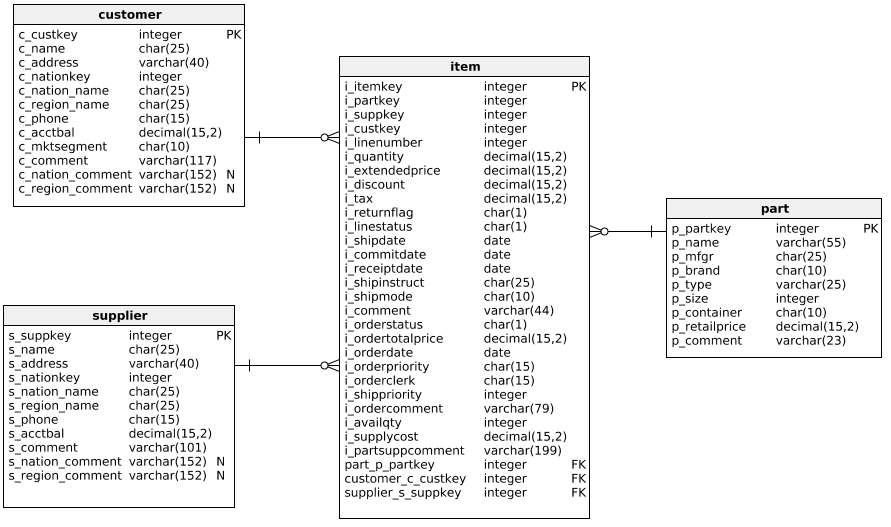
\includegraphics[width=\textwidth]{star}
	\caption{Esquema do ambiente star}
	\label{fig:star}
\end{figure*}

As modificações no modelo do ambiente \textit{snowflake} se fundamentaram na criação de um modelo como o apresentado pela modelagem \textit{star}, com uma entidade fato central descrita por dimensões, eliminando-se tabelas subdimensão e unindo atributos fato de diferentes entidades. O modelo é ilustrado na Figura \ref{fig:star}.
 
A primeira modificação no modelo original foi a exclusão das entidades subdimensão \textit{nation} e \textit{region}. Incluiu-se portanto os atributos \texttt{n\_name, n\_comment, r\_name} e \texttt{r\_comment} nas entidades \textit{supplier} e \textit{customer}. 

Com a intenção de criar um único fato no esquema denormalizado, observou-se (i) a possibilidade de unir as entidades \textit{lineitem} e \textit{orders} em uma única entidade renomeada \textit{item}. Isto também eliminaria algumas junções realizadas entre as duas entidades nas consultas do TPC-H. Também se nota que (ii) as entidades \textit{part} e \textit{supplier} se relacionam com \textit{lineitem} através da entidade intermediária \textit{partsupp}. Optou-se assim por incluir os atributos de \textit{partsupp} na nova entidade \textit{item}, excluindo a primeira do esquema e mantendo o relacionamento de \textit{supplier} e \textit{part} diretamente com \textit{item}.

O esquema final agora possui apenas uma entidade fato: \textit{item}; e três entidades dimensão: \textit{part}, \textit{customer} e \textit{supplier}. Os dados presentes nas entidades são do mesmo tipo descritos na seção anterior. Tanto as consultas quanto os dados foram modificados de forma a se adequar ao novo esquema.

Como o ambiente modificado não faz parte do TPC-H, o DBGen não tem suporte à geração automática de dados segundo a nova modelagem. Com isso, para que seja feita a nova geração de dados optou-se por uma abordagem que conta com o auxilio dos dados já gerados pelo DBGen. Após populados os registros no banco original são executadas junções a fim de projetar os atributos requeridos por cada entidade do modelo \textit{star}. O resultado desta projeção é inserido nas tabelas da modelagem adaptada. O mesmo se aplica às consultas, como o QGen não têm suporte à diferentes modelagens, adaptou-se manualmente as 22 consultas.

\subsection{O Processo de Avaliação}

Após a geração dos arquivos é criado em cada SGBD um esquema correspondente às classes utilizadas, tanto para o ambiente \textit{snowflake} quanto para o \textit{star}. Cada SGBD é então executado sobre os dois ambientes propostos. Em cada ambiente será executado o teste de desempenho, que consiste de duas execuções: o teste de força e o teste de vazão. O tempo resultante de cada etapa é utilizado para calcular o desempenho do SGBD, utilizando a unidade de medida \textit{QphH@Size} -- quantidade de consultas executadas por hora dada uma classe de tamanho de banco de dados. As execuções em geral são compostas por:

\begin{itemize}
	\item \textit{SF}, que representa a classe do banco de dados.
	\item \textit{$Q_{i}$}, que representa uma consulta, onde \mbox{$1 \le i \le 22$}.
	\item \textit{S}, que define o número de sessões de consulta do Teste de Vazão.
	\item \textit{s}, que representa uma dada sessão, onde \mbox{$1 \le s \le S$}.
	\item \textit{$T_{s}$}, que representa o tempo, em segundos, resultante do processo inteiro.
	\item \textit{$RF_{j}$}, que representa uma função de atualização (FA) onde:
		\begin{itemize}
		    \item FA1: inserção de novos registros. São gerados novos dados para as tabelas fato com quantidade proporcional ao fator de escala. 
		    \item FA2: remoção de registros antigos. São removidos dados antigos das tabelas fato, e o número de registros deletados deve ser igual ao número de registros inseridos. Note que não necessariamente são removidos os dados inseridos na FA1.
		\end{itemize}
\end{itemize}

\subsection{Teste de Força}
\label{power_test}
O Teste de Força objetiva medir a taxa de consultas por hora do sistema com um único usuário ativo. Neste teste é criada uma única sessão com o respectivo SGBD e as seguintes instruções são executadas:

\begin{enumerate}
	\item Execução da FA1.
	\item Execução de cada consulta proposta pelo TPC-H, ou adaptada, de forma sequencial uma única vez até a última consulta.
	\item Execução da FA2.
\end{enumerate}

Será armazenado ao fim do teste o tempo em segundos resultante de cada consulta, bem como o tempo de execução de cada função. Este resultado será utilizado na Equação \ref{eq:1}.

\begin{myequation}%
\label{eq:1}
{\scriptstyle Power = } {\scriptstyle \frac{3600 * SF}{\sqrt[24]{\prod_{i = 2}^{i = 22}Q(i, 0) * \prod_{j = 1}^{j = 2}RF(j, 0)}}} %
\end{myequation}
%

\subsection{Teste de Vazão}
\label{through_test}
Este teste mede a capacidade do sistema de processar a maior quantidade possível de consultas no menor intervalo de tempo. Aqui o TPC-H exige um número mínimo de sessões de consulta de acordo com a classe de tamanho do banco de dados, como mostra a Tabela \ref{min_sessions}.

\begin{table}[htpb]
\centering
\caption{Número mínimo de sessões para uma classe de banco de dados}
\label{min_sessions}
\begin{tabular}{|c|c|}
\hline
\multicolumn{1}{|c|}{\textbf{Classe do Banco de Dados}} & \textbf{Número de Sessões} \\ \hline
1 GB                                      & 2                            \\ \hline
10 GB                                      & 3                          \\ \hline
30 GB                                        & 4                             \\ \hline
100 GB                                        & 5                             \\ \hline
300 GB                                        & 6                             \\ \hline
1000 GB                                        & 7                             \\ \hline
3000 GB                                        & 8                             \\ \hline
10000 GB                                        & 9                             \\ \hline
30000 GB                                        & 10                             \\ \hline
100000 GB                                        & 11                             \\ \hline
\end{tabular}
\end{table}

É criada uma sessão para executar as funções e \textit{N} sessões para executar as consultas, de acordo com a Tabela \ref{min_sessions}. As instruções são executadas concorrentemente. Para a sessão das funções, as seguintes instruções são executadas:

\begin{itemize}
	\item A FA1 e FA2 deverão ser executadas sequencialmente \textit{N} vezes, onde \textit{N} é o número de sessões para a execução de consultas.
	\item Para cada sessão de consultas, cada consulta será executada sequencialmente até a última.
\end{itemize}

Ao fim do teste, é armazenado o tempo em segundos da execução do processo inteiro. O processo inicia quando a primeira sessão, seja de consulta ou de função, executa sua instrução e finaliza quando a última sessão recebe uma resposta. O resultado é utilizado para calcular o desempenho dos SGBD para o teste conforme a Equação \ref{eq:2}.

\begin{myequation}%
\label{eq:2}
{\scriptstyle Throughput} = \frac{S * 22 * 3600}{T_s * SF} %
\end{myequation}
%

O resultado dos cálculos de força e vazão serão ponderados de maneira uniforme para calcular o desempenho final do SGBD de acordo com a fórmula:

\begin{myequation}%
\label{eq:3}
{ \scriptstyle QphH@Size = \sqrt{Power * Throughput} } %
\end{myequation}
%

\section{Resultados e Discussão}

O experimento para análise de desempenho foi feito sob uma base de dados de 1GB. Além dos SGBD PostgreSQL e MonetDB, considerou-se previamente a inclusão do MySQL nos testes de desempenho devido a sua popularidade. Seu uso foi logo descartado em virtude da notória discrepância de tempo para carga de dados se comparado aos outros dois. Essa diferença pode ser vista na Tabela \ref{tab:carga}, que mostra o tempo da inserção de dados em segundos, e é ilustrada na Figura \ref{fig:carga}.


\begin{table}[htpb]
\centering
\caption{Carga de Dados}
\label{tab:carga}
\begin{tabular}{@{}lccc@{}}
\toprule
          & MySQL  & PostgreSQL & MonetDB \\ \midrule
Snowflake & 205,49 & 84,688     & 33,54   \\
Star      & 317    & 170        & 61      \\ \bottomrule
\end{tabular}
\end{table}

\begin{figure}[htpb]
  \centering
  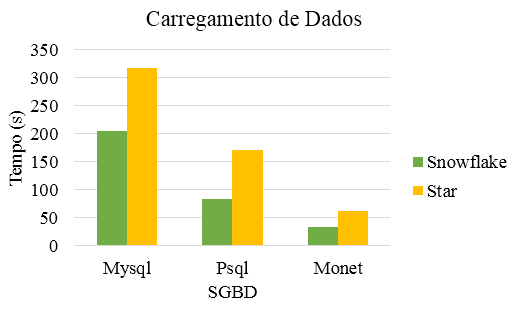
\includegraphics[width=7cm]{carregamento}
  \caption{Gráfico da carga de dados}
  \label{fig:carga}
\end{figure}

Para se obter um melhor desempenho no carregamento de dados as restrições de chave foram realizadas após a inserção dos dados nos SGBDs. Caso a restrição fosse feita na criação do banco a cada novo registro inserido a chave primária seria verificada. Esta carga de dados também foi realizada através dos SGBD de forma direta, sem o uso de drivers e outras ferramentas que possam atuar como cliente para conectar-se ao banco, assim evitando incluir o tempo de latência destas no resultado.

Logo ao analisar os resultados de carregamento de dados nota-se que um banco denormalizado apresenta certa demora na inserção de dados em relação a um normalizado. Isso se dá por causa da redundância de dados existente neste tipo de modelo, fazendo com que existam mais atributos duplicados em uma mesma entidade; aumentando o tamanho das entidades a serem inseridas. Toma-se como exemplo a entidade \textit{nation}: no modelo \textit{snowflake} ela é uma tabela subdimensão e possui 25 registros apenas, enquanto que no modelo denormalizado ela faz parte das tabelas dimensão \textit{supplier} e \textit{customer}, fazendo com que estas duas entidades tenham mais bytes armazenados. A Tabela \ref{tab:tamanho} mostra o tamanho das entidades em cada modelo. Note que \textit{part} não tem seu valor alterado por não sofrer alteração entre as modelagens.

\begin{table}[htpb]
\centering
\caption{Tamanho em bytes das entidades}
\label{tab:tamanho}
\begin{tabular}{@{}lcc@{}}
\toprule
              & Snowflake & Star       \\ \midrule
Supplier      & 1.409.184   & 2.990.430    \\
Customer      & 24.346.144  & 48.055.517   \\
Part          & 24.135.125  & 24.135.125   \\
Lineitem/Item & 759.863.287 & 2.226.620.122 \\ \bottomrule
\end{tabular}
\end{table}

Após a inserção de dados somente os SGBD PostgreSQL e MonetDB foram utilizados para o benchmarking.  Optou-se por desenvolver o processo do TPC-H utilizando o driver JDBC\footnote{http://www.oracle.com/technetwork/java/javase/jdbc/index.html} pela simplificação que seu uso traz ao desenvolvimento de aplicações e por dar suporte à vários SGBD. Porém, há que considerar a latência do driver no teempo de execução devido à ponte entre a chamada de um procedimento do JDBC até a conexão com o SGBD. 

A execução começa com o teste de força seguido imediatamente do teste de vazão, conforme as Equações \ref{eq:1} e \ref{eq:2}. Logo nos resultados apresentados por estas execuções nota-se a diferença de desempenho do PostgreSQL e do MonetDB -- atentando-se para o fato de que quanto maior o valor, melhor. As Tabelas \ref{tab:força} e \ref{tab:vazão} mostram os resultados obtidos em cada execução em consultas por hora (\textit{qph}).

\begin{table}[htpb]
\centering
\caption{Teste de Força}
\label{tab:força}
\begin{tabular}{@{}lccc@{}}
\toprule
          & PostgreSQL & MonetDB \\ \midrule
Snowflake & 4,5711     & 46,5462   \\
Star      & 2,2154        & 53,0620     \\ \bottomrule
\end{tabular}
\end{table}

\begin{table}[htpb]
\centering
\caption{Teste de Vazão}
\label{tab:vazão}
\begin{tabular}{@{}lccc@{}}
\toprule
          & PostgreSQL & MonetDB \\ \midrule
Snowflake & 1566,7346     & 5524,4257   \\
Star      & 785,1225        & 7243,2810    \\ \bottomrule
\end{tabular}
\end{table}

Tendo os resultados do teste de força e vazão, calculou-se o resultado final do benchmark para se obter a quantidade de consultas executadas por hora no sistema, conforme a Equação \ref{eq:3}. A Tabela \ref{tab:resultado} mostra o resultado final em \textit{qph} e a Figura \ref{fig:resultado} ilustra graficamente os dados da tabela.

\begin{table}[htpb]
\centering
\caption{Resultado do benchmark -- QphH@1GB}
\label{tab:resultado}
\begin{tabular}{@{}lccc@{}}
\toprule
          & PostgreSQL & MonetDB \\ \midrule
Snowflake & 84,6271     & 507,0913   \\
Star      & 41,7061        & 619,9545    \\ \bottomrule
\end{tabular}
\end{table}

\begin{figure}[htpb]
  \centering
  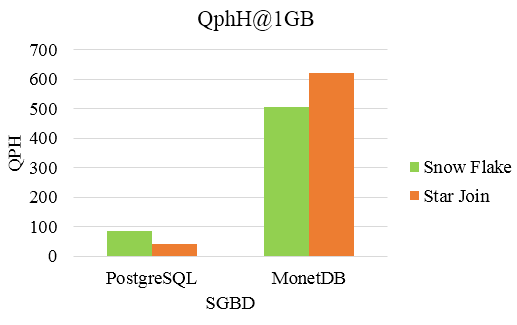
\includegraphics[width=7cm]{resultado}
  \caption{Gráfico do resultado final}
  \label{fig:resultado}
\end{figure}

Analisando de fato os resultados do benchmark, de maneira geral o SGBD que obteve melhores resultados foi o MonetDB, desde a execução isolada dos testes de força e vazão até o resultado final. Em relação aos ambientes o MonetDB denormalizado apresentou resultados melhores, o que reforça o uso de SGBD NoSQL em ambientes denormalizados sob um grande volume de dados. Se tomar apenas o SGBD, o desempenho baixo do PostgreSQL era esperado ao se comparar com um banco colunar devido ao armazenamento e leitura aprimorados do MonetDB, tanto para um ambiente normalizado quanto para um denormalizado. 

Comparando os resultados do PostgreSQL de maneira isolada percebe-se que a lógica nos resultados não é a mesma do MonetDB, e que outra teoria é reforçada: a de que SGBD relacionais estão fortemente atrelados a modelagens mais normalizadas e são otimizados para se adequar melhor a esta modelagem.


\section{Conclusão e Trabalhos Futuros}

O SGBD MonetDB foi superior em quase 500\% do PostgreSQL para o ambiente \textit{snowflake}, representando uma diferença de 6 vezes no resultado final. Também foi melhor em mais de 1000\% ao relacional na modelagem \textit{star}, tendo quase 15 vezes o valor do PostgreSQL. Estes resultados como um todo corroboram a ideia de que o uso de SGBD NoSQL traz vantagens a ambientes OLAP, por adaptar-se melhor à modelagem comumente utilizada por Data Warehouses.

Sugere-se ainda a inclusão de mais SGBD NoSQL, fazendo um comparativo entre SGBD de diferentes classes a fim de analisar seu comportamento sob um ambiente empresarial e também qual impacto a ausência de SQL pode trazer ao desempenho, visto que SGBD como o MongoDB e o Neo4J utilizam uma linguagem orientada a documentos e a grafos, respectivamente. Também como trabalho futuro, será realizada a aplicação dos resultados do estudo em empresas que não possuam uma modelagem fortemente denormalizada e tampouco utilizem NoSQL, a fim de averiguar os resultados encontrados pelo benchmark.


% An example of a floating figure using the graphicx package.
% Note that \label must occur AFTER (or within) \caption.
% For figures, \caption should occur after the \includegraphics.
% Note that IEEEtran v1.7 and later has special internal code that
% is designed to preserve the operation of \label within \caption
% even when the captionsoff option is in effect. However, because
% of issues like this, it may be the safest practice to put all your
% \label just after \caption rather than within \caption{}.
%
% Reminder: the "draftcls" or "draftclsnofoot", not "draft", class
% option should be used if it is desired that the figures are to be
% displayed while in draft mode.
%
%\begin{figure}[!t]
%\centering
%\includegraphics[width=2.5in]{myfigure}
% where an .eps filename suffix will be assumed under latex, 
% and a .pdf suffix will be assumed for pdflatex; or what has been declared
% via \DeclareGraphicsExtensions.
%\caption{Simulation results for the network.}
%\label{fig_sim}
%\end{figure}

% Note that the IEEE typically puts floats only at the top, even when this
% results in a large percentage of a column being occupied by floats.


% An example of a double column floating figure using two subfigures.
% (The subfig.sty package must be loaded for this to work.)
% The subfigure \label commands are set within each subfloat command,
% and the \label for the overall figure must come after \caption.
% \hfil is used as a separator to get equal spacing.
% Watch out that the combined width of all the subfigures on a 
% line do not exceed the text width or a line break will occur.
%
%\begin{figure*}[!t]
%\centering
%\subfloat[Case I]{\includegraphics[width=2.5in]{box}%
%\label{fig_first_case}}
%\hfil
%\subfloat[Case II]{\includegraphics[width=2.5in]{box}%
%\label{fig_second_case}}
%\caption{Simulation results for the network.}
%\label{fig_sim}
%\end{figure*}
%
% Note that often IEEE papers with subfigures do not employ subfigure
% captions (using the optional argument to \subfloat[]), but instead will
% reference/describe all of them (a), (b), etc., within the main caption.
% Be aware that for subfig.sty to generate the (a), (b), etc., subfigure
% labels, the optional argument to \subfloat must be present. If a
% subcaption is not desired, just leave its contents blank,
% e.g., \subfloat[].


% An example of a floating table. Note that, for IEEE style tables, the
% \caption command should come BEFORE the table and, given that table
% captions serve much like titles, are usually capitalized except for words
% such as a, an, and, as, at, but, by, for, in, nor, of, on, or, the, to
% and up, which are usually not capitalized unless they are the first or
% last word of the caption. Table text will default to \footnotesize as
% the IEEE normally uses this smaller font for tables.
% The \label must come after \caption as always.
%
%\begin{table}[!t]
%% increase table row spacing, adjust to taste
%\renewcommand{\arraystretch}{1.3}
% if using array.sty, it might be a good idea to tweak the value of
% \extrarowheight as needed to properly center the text within the cells
%\caption{An Example of a Table}
%\label{table_example}
%\centering
%% Some packages, such as MDW tools, offer better commands for making tables
%% than the plain LaTeX2e tabular which is used here.
%\begin{tabular}{|c||c|}
%\hline
%One & Two\\
%\hline
%Three & Four\\
%\hline
%\end{tabular}
%\end{table}


% Note that the IEEE does not put floats in the very first column
% - or typically anywhere on the first page for that matter. Also,
% in-text middle ("here") positioning is typically not used, but it
% is allowed and encouraged for Computer Society conferences (but
% not Computer Society journals). Most IEEE journals/conferences use
% top floats exclusively. 
% Note that, LaTeX2e, unlike IEEE journals/conferences, places
% footnotes above bottom floats. This can be corrected via the
% \fnbelowfloat command of the stfloats package.




% trigger a \newpage just before the given reference
% number - used to balance the columns on the last page
% adjust value as needed - may need to be readjusted if
% the document is modified later
%\IEEEtriggeratref{8}
% The "triggered" command can be changed if desired:
%\IEEEtriggercmd{\enlargethispage{-5in}}

% references section


\bibliographystyle{IEEEtran}
\bibliography{references.bib}

\end{document}